\documentclass[aspectratio=169,10pt]{beamer}
\usepackage[T1]{fontenc}
\usepackage{lmodern}
\usepackage{amsmath,amssymb}
\usepackage{graphicx}
\usepackage{tikz}
\usetikzlibrary{positioning,arrows.meta,decorations.pathmorphing}
\graphicspath{{figures/}{figures/lesson/}}
\newcommand{\norm}[1]{\lVert #1 \rVert}

\definecolor{osuorange}{HTML}{DC4405}
\definecolor{osudark}{HTML}{1A1A1A}
\definecolor{osugray}{HTML}{4D4D4D}

\usetheme{default}
\setbeamercolor{title}{fg=osuorange}
\setbeamercolor{frametitle}{fg=white,bg=osuorange}
\setbeamercolor{structure}{fg=osuorange}
\setbeamercolor{normal text}{fg=osudark}
\setbeamercolor{itemize item}{fg=osuorange}
\setbeamercolor{itemize subitem}{fg=osuorange}
\setbeamerfont{frametitle}{series=\bfseries,size=\large}
\setbeamerfont{title}{series=\bfseries}
\setbeamertemplate{itemize item}{\raisebox{0.25ex}{\footnotesize\textcolor{osuorange}{$\blacktriangleright$}}}
\setbeamertemplate{itemize subitem}{\textcolor{osuorange}{\textbullet}}
\setbeamertemplate{navigation symbols}{}
\setbeamertemplate{footline}{%
  \hfill\textcolor{osugray}{\footnotesize\insertframenumber}\hspace{1.2em}\vspace{0.8em}}
\setbeamertemplate{frametitle}{%
  \vspace{0.4em}\hspace{0.2em}\textcolor{osuorange}{\bfseries\insertframetitle}\par
  \vspace{-0.2em}{\color{osuorange}\rule{\linewidth}{1.2pt}}}

% tighter list spacing
\setlength{\leftmargini}{1.2em}
\setbeamertemplate{itemize/enumerate body begin}{\itemsep=2pt}

\title{\textbf{Recovering the Hidden Digit, Part II}}
\subtitle{Diffusion-prior posterior sampling for ERT}
\author{Travis Whitney \quad Cole Seifert \quad Alexander Nutt}
\institute{AI 539, Oregon State University}
\date{Project 2 Competition, Spring 2026}

\begin{document}

\begin{frame}
  \titlepage
\end{frame}

%==============================================================
\begin{frame}{Same problem, new rule}
The physics from Project 1 hasn't changed. We still have a hidden
$28 \times 28$ digit, a list of 1900 boundary voltage readings, and
the forward simulator $F$. The job is still to work backward from the
readings to the digit.

\vspace{0.6em}
What changed is the rule on the prior. In Project 1 we used the 60{,}000
MNIST training images as a lookup table. For Project 2 the prior has to
be a diffusion model. A diffusion model is a neural network that learned
what a digit looks like by practicing on the MNIST set. We can ask it to
draw a fresh digit, but it does not know about our voltage readings.

\vspace{0.6em}
The rest of this talk is how we combined a diffusion model with the ERT
measurements. The final misfit is
\textcolor{osuorange}{$\mathbf{6.16 \times 10^{-13}}$}, recovering a
tilted 5.
\end{frame}

%==============================================================
\begin{frame}{The pipeline}
\centering
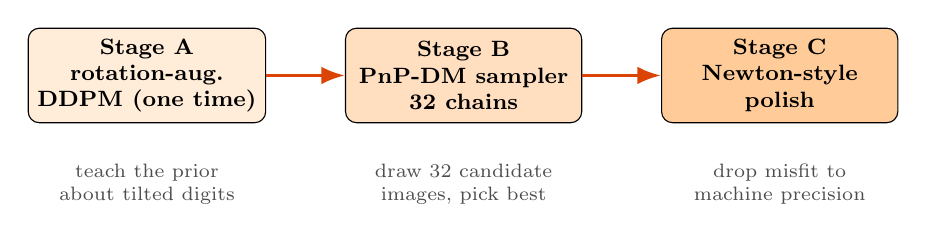
\begin{tikzpicture}[node distance=0.4cm and 1.0cm, every node/.style={align=center}]
\node[draw, rounded corners, fill=orange!15, minimum width=3.0cm, minimum height=1.2cm,
      font=\footnotesize\bfseries] (A) {Stage A\\rotation-aug.\\DDPM (one time)};
\node[draw, rounded corners, fill=orange!25, minimum width=3.0cm, minimum height=1.2cm,
      right=of A, font=\footnotesize\bfseries] (B) {Stage B\\PnP-DM sampler\\32 chains};
\node[draw, rounded corners, fill=orange!40, minimum width=3.0cm, minimum height=1.2cm,
      right=of B, font=\footnotesize\bfseries] (C) {Stage C\\Newton-style\\polish};
\draw[-{Latex[length=3mm]}, very thick, osuorange] (A) -- (B);
\draw[-{Latex[length=3mm]}, very thick, osuorange] (B) -- (C);
\node[below=0.4cm of A, font=\scriptsize, color=osugray] {teach the prior\\about tilted digits};
\node[below=0.4cm of B, font=\scriptsize, color=osugray] {draw 32 candidate\\images, pick best};
\node[below=0.4cm of C, font=\scriptsize, color=osugray] {drop misfit to\\machine precision};
\end{tikzpicture}

\vspace{1.5em}
Stage A is a one-time setup. After that, every run goes through Stage B
and Stage C. Total wall time on a MacBook is about eight minutes.
\end{frame}

%==============================================================
\begin{frame}{What a diffusion model lets us do}
\begin{columns}[T]
\column{0.55\textwidth}
\vspace{0.4em}
{\small A diffusion model is trained to look at a noisy image and predict
the noise that was added. Once it can do that, simple algebra gives us a
guess at the clean image underneath:}
\[
\hat x_0 \;=\;
\frac{x_t \,-\, \sqrt{1 - \bar\alpha_t}\,\varepsilon_\theta(x_t, t)}{\sqrt{\bar\alpha_t}}.
\]
\vspace{-0.3em}

{\small So at any moment along a noisy chain, the network gives us its
best guess at the clean digit underneath. At high noise the guess is
fuzzy. At low noise it is sharp. Every method here leans on that one
identity.}

\column{0.45\textwidth}
\centering
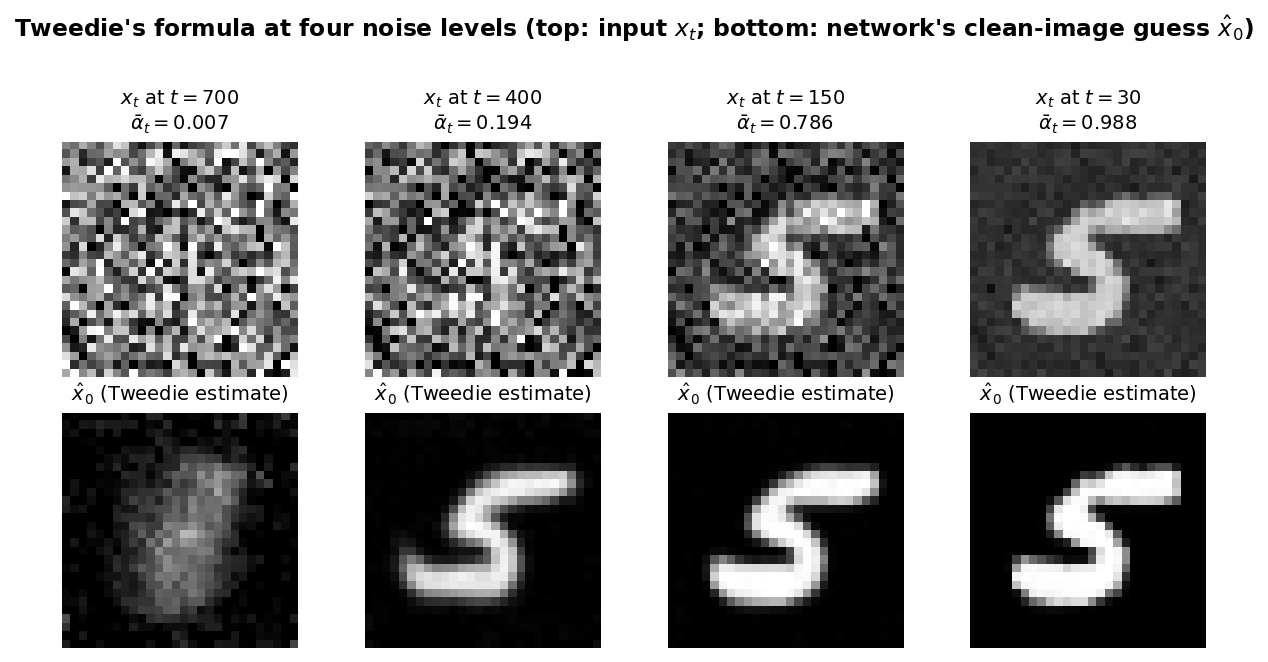
\includegraphics[width=\linewidth]{fig05_tweedie_strip.png}\\
{\scriptsize\color{osugray} Top: a noisy input at four noise levels.
Bottom: the network's clean-image guess at each.}
\end{columns}
\end{frame}

%==============================================================
\begin{frame}{What we tried first}
\footnotesize

\textbf{The idea.} Train a diffusion model on the 60{,}000 MNIST digits
so it knows what handwritten digits look like. Then, instead of asking
it to draw random digits, steer its drawing process at every step using
the ERT measurements. The result should be a digit that looks realistic
and matches the data.

\vspace{0.4em}
The steering works by asking, at every step, ``if this were the final
image, how far off would the predicted voltages be from what we
measured?'' Then nudge the image to reduce that mismatch.

\vspace{0.4em}
This is the standard recipe in the literature. It is called DPS, short
for Diffusion Posterior Sampling.

\vspace{0.4em}
\textbf{What happened.} We ran this five separate times from different
random starting noise.

\vspace{0.5em}
\begin{center}
{\large\textcolor{osuorange}{\textbf{Four of the five runs agreed the digit is a 4.}}}
\end{center}

\vspace{0.2em}
\centering
{\scriptsize\color{osugray}
Project 1 already showed the digit is a 5. So this approach gave us the
wrong answer, consistently.}
\end{frame}

%==============================================================
\begin{frame}{Why it got the wrong digit}
\begin{columns}[T]
\column{0.52\textwidth}
\vspace{0.2em}
\footnotesize
Two things broke at once.

\vspace{0.4em}
\begin{itemize}\itemsep=4pt
\item The little nudge at each step is in the direction of the data
  gradient. That gradient is dominated by directions the boundary
  sensors hardly see, so most of the nudge goes to waste.
\item The drawing process only has about 100 steps. A hundred weak
  nudges are not enough to override the prior's pull toward the most
  common-looking digit.
\end{itemize}

\vspace{0.4em}
The chain commits early to whatever upright digit shape is closest
to the data. For this measurement vector, that was a 4.

\column{0.48\textwidth}
\centering
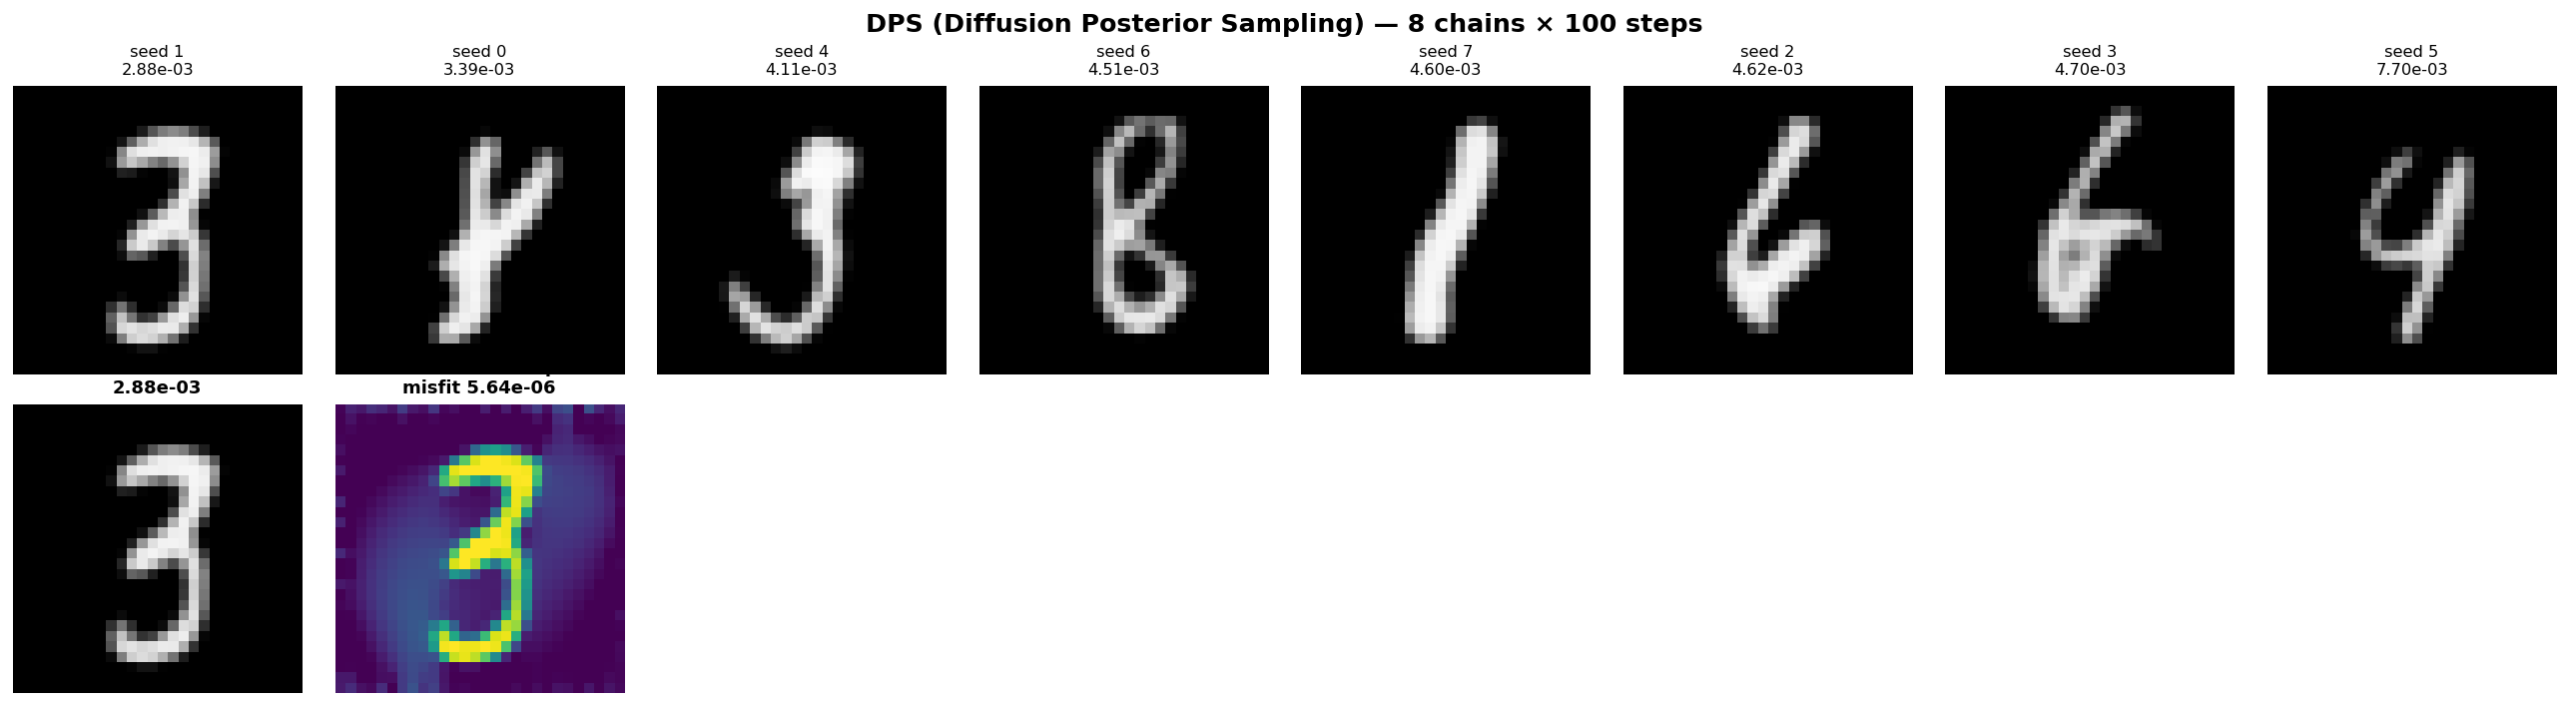
\includegraphics[width=\linewidth]{dps_chains.png}\\
{\scriptsize\color{osugray} Eight chains from our DPS run, each
locked onto a wrong digit (3, 4, 6, 8). No 5 in sight.}
\end{columns}
\end{frame}

%==============================================================
\begin{frame}{The fix: split the work between two variables}
\begin{columns}[T]
\column{0.55\textwidth}
\vspace{0.2em}
\footnotesize
DPS asks one variable to do two jobs at once: look like a digit, and
fit the data. The two pulls compromise on every step, and the smaller
one loses.

\vspace{0.5em}
Instead, introduce a second variable. Call them $x$ and $z$. Give them
separate jobs:

\vspace{0.3em}
\begin{itemize}\itemsep=3pt
\item $x$ only has to look like a digit.
\item $z$ only has to fit the measurements.
\item A soft penalty keeps $z$ near $x$.
\end{itemize}

\vspace{0.5em}
Then alternate. Update $z$ to fit the data. Update $x$ to look like a
digit. Repeat. Each update does one thing well.

\vspace{0.4em}
This sampler is called PnP-DM (Wu et al., NeurIPS 2024). We run 80
alternations per chain, 32 chains in parallel.

\column{0.45\textwidth}
\centering
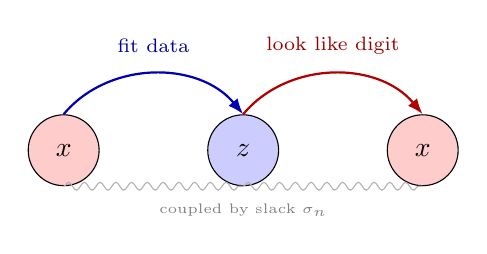
\begin{tikzpicture}[scale=0.95]
\node[draw, circle, fill=red!20, minimum size=0.9cm] (x1) at (0, 0) {\(x\)};
\node[draw, circle, fill=blue!20, minimum size=0.9cm] (z1) at (2.4, 0) {\(z\)};
\node[draw, circle, fill=red!20, minimum size=0.9cm] (x2) at (4.8, 0) {\(x\)};
\draw[-{Latex[length=2mm]}, thick, blue!70!black]
  (x1.north) .. controls (0.6, 1.2) and (1.8, 1.2) .. (z1.north);
\node[blue!60!black, font=\scriptsize, align=center] at (1.2, 1.4)
  {fit data};
\draw[-{Latex[length=2mm]}, thick, red!70!black]
  (z1.north) .. controls (3.0, 1.2) and (4.2, 1.2) .. (x2.north);
\node[red!60!black, font=\scriptsize, align=center] at (3.6, 1.4)
  {look like digit};
\draw[gray!60, decorate, decoration={snake, amplitude=0.5mm, segment length=2mm}] (x1.south) -- (z1.south);
\draw[gray!60, decorate, decoration={snake, amplitude=0.5mm, segment length=2mm}] (z1.south) -- (x2.south);
\node[font=\tiny, gray] at (2.4, -0.8) {coupled by slack \(\sigma_n\)};
\end{tikzpicture}
\end{columns}
\end{frame}

%==============================================================
\begin{frame}{Why the data step works this time}
\footnotesize
The data step picks the $z$ that fits the measurements while staying
near the current $x$. DPS just takes a gradient step in this objective.
We instead take one Gauss-Newton step, the textbook move for nonlinear
least-squares.

\vspace{0.5em}
Gauss-Newton approximates the forward map by its tangent plane at the
current point. That makes the data-fit objective quadratic, with a
closed-form minimum. We solve one small linear system and jump straight
to that minimum:
\[
\Bigl(\tfrac{1}{\sigma_{\text{meas}}^{2}}\,J^{\top} J + \tfrac{1}{\sigma_n^{2}}\,I\Bigr)\,\Delta
\;=\; -\tfrac{1}{\sigma_{\text{meas}}^{2}}\,J^{\top} r + \tfrac{1}{\sigma_n^{2}}\,(x - z),
\quad z \leftarrow z + \Delta.
\]
\vspace{-0.4em}

\textbf{Difference from DPS.} DPS takes one small step in the gradient
direction. Gauss-Newton solves the local data-fit problem outright. On
an ill-conditioned Jacobian like ours, one Gauss-Newton step does the
work of dozens of gradient steps.

\vspace{0.3em}
\centering
\textcolor{osuorange}{That extra strength is what commits the chain to the right digit.}
\end{frame}

%==============================================================
\begin{frame}{One chain, six frames: noise becomes a 5}
\centering
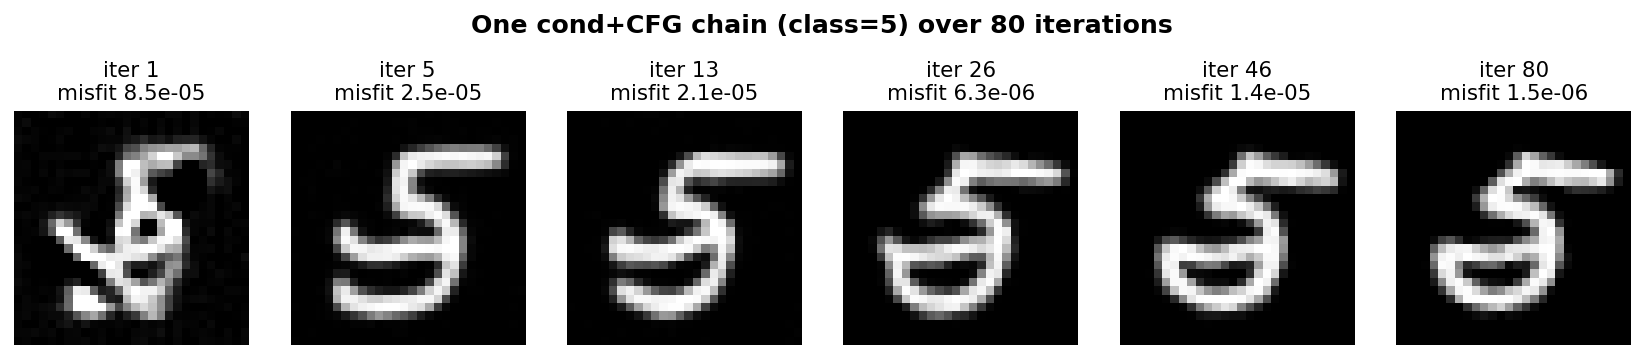
\includegraphics[width=0.98\linewidth]{fig_denoising_progression.png}

\vspace{0.8em}
{\footnotesize
\textbf{Reading left to right.} At iteration 1 the image is essentially
random noise. By iteration 5 a digit shape is forming. By iteration 26
the digit identity (a 5) is settled, though the strokes are still a bit
smudged. By iteration 80 the chain has converged to a clean tilted 5
with misfit around $10^{-7}$. Every other chain looks similar.}
\end{frame}

%==============================================================
\begin{frame}{One more piece: rotation augmentation}
\begin{columns}[T]
\column{0.55\textwidth}
\vspace{0.2em}
\footnotesize
The pretrained MNIST diffusion model has only seen upright digits
during training. Our truth is a 5 tilted by about $7.5$ degrees. During
PnP-DM the prior step keeps nudging back toward upright, while the data
step pulls toward tilted. Without intervention the prior wins.

\vspace{0.5em}
The fix is to keep training the diffusion model a little longer, but on
rotated copies of the MNIST digits. Five epochs of this on a MacBook
takes about twenty minutes.

\vspace{0.5em}
After the extra training, the model thinks tilted digits are just as
normal as upright ones. The prior step stops fighting the data, and the
chain converges to the truth.

\column{0.45\textwidth}
\centering
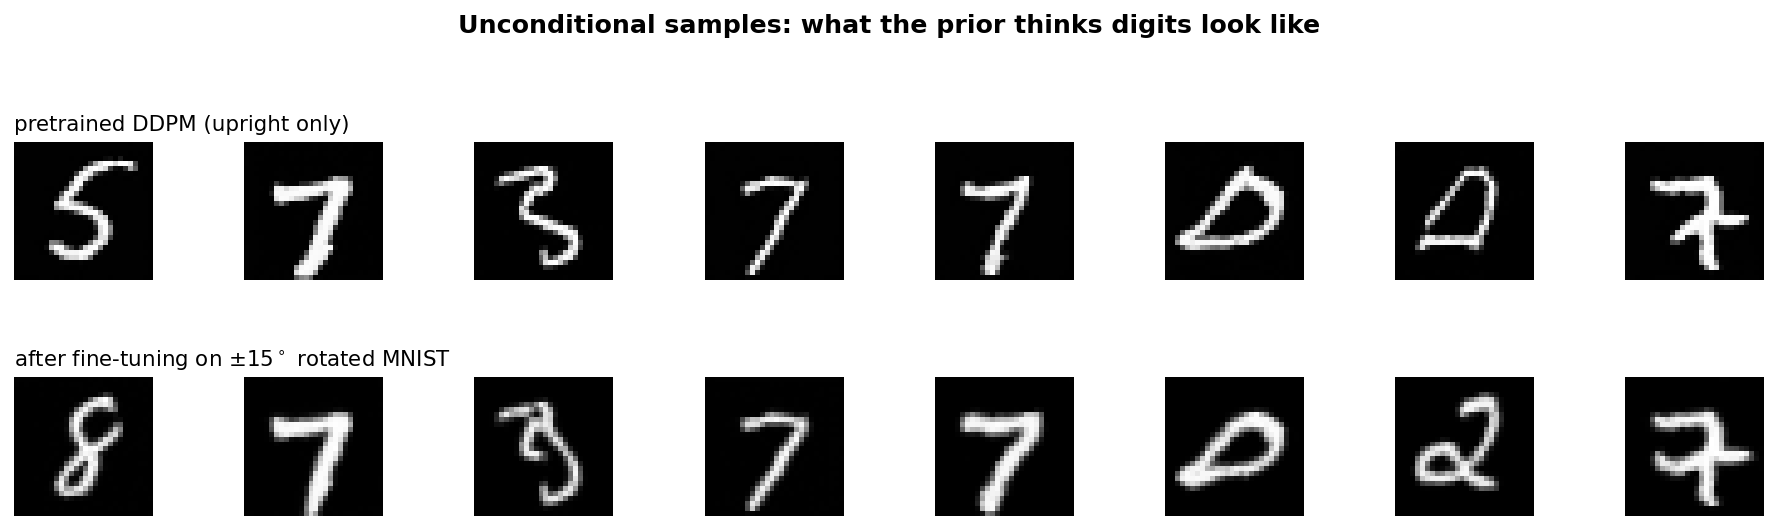
\includegraphics[width=\linewidth]{fig10_pretrained_vs_finetuned.png}\\
{\scriptsize\color{osugray} Top row: random digits from the pretrained
model. Bottom row: random digits from the same model after the extra
rotation training.}
\end{columns}
\end{frame}

%==============================================================
\begin{frame}{Finishing the job: a Newton-style polish}
\begin{columns}[T]
\column{0.50\textwidth}
\vspace{0.1em}
\footnotesize
After PnP-DM the best chain has misfit about $1.8 \times 10^{-7}$.
We know the digit is right. The rest is a local optimization on
the pixels.

\vspace{0.4em}
Project 1's polish was gradient descent. It converges linearly, and
the steps get tinier as we approach the optimum.

\vspace{0.4em}
Instead we use a Newton-style step, which accounts for the curvature
of the data-fit landscape. Each step roughly squares the error, so a
handful of steps drops the misfit many orders of magnitude. We hit
the float64 floor in about 25 seconds.

\vspace{0.3em}
\textcolor{osuorange}{\textbf{Final misfit: $\mathbf{6.16 \times 10^{-13}}$.}}

\column{0.50\textwidth}
\centering
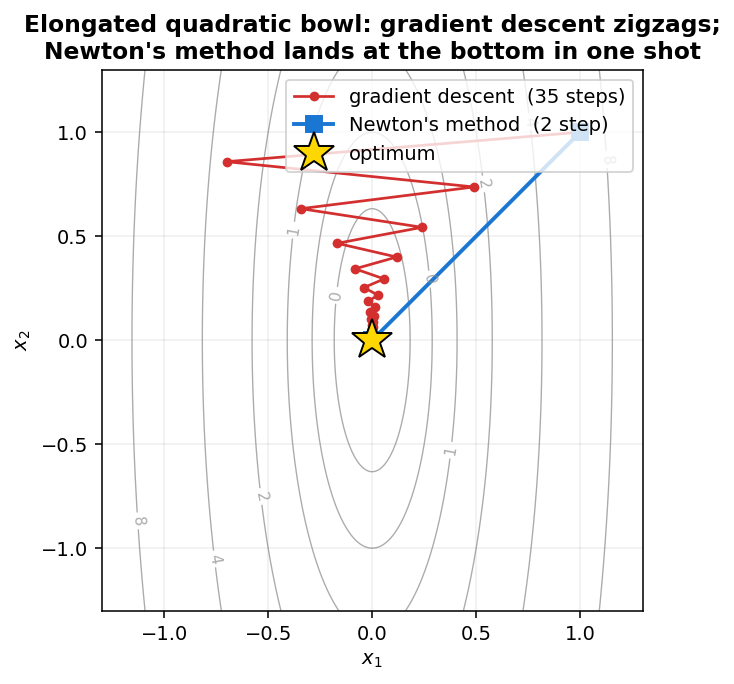
\includegraphics[width=\linewidth]{fig11_gd_vs_newton.png}\\
{\scriptsize\color{osugray} GD zigzags; Newton jumps to the bottom.}
\end{columns}
\end{frame}

%==============================================================
\begin{frame}{What we recovered}
\begin{columns}[T]
\column{0.55\textwidth}
\centering

\includegraphics[width=\linewidth]{fig12_recovered_sigma.png}
\column{0.45\textwidth}
\vspace{0.8em}
\footnotesize
The recovered digit is a \textbf{5}, tilted by about $7.5$ degrees. The
final misfit is
\textcolor{osuorange}{$\boldsymbol{6.16 \times 10^{-13}}$}.

\vspace{0.5em}
That is roughly $163{,}000$ times tighter than Project 1's
rotation-aware result on the same data. The pipeline ran all the way
down to the limit of double-precision arithmetic.

\vspace{0.5em}
{\color{osugray} Most of that big multiplier comes from the polish, not
from the diffusion. The diffusion did its job by putting us in the
right digit basin. Once there, the Newton-style polish beat Project 1's
gradient polish by about five orders of magnitude.}
\end{columns}
\end{frame}

%==============================================================
\begin{frame}{Same method on 10 unseen digits: 9 out of 10}
\centering
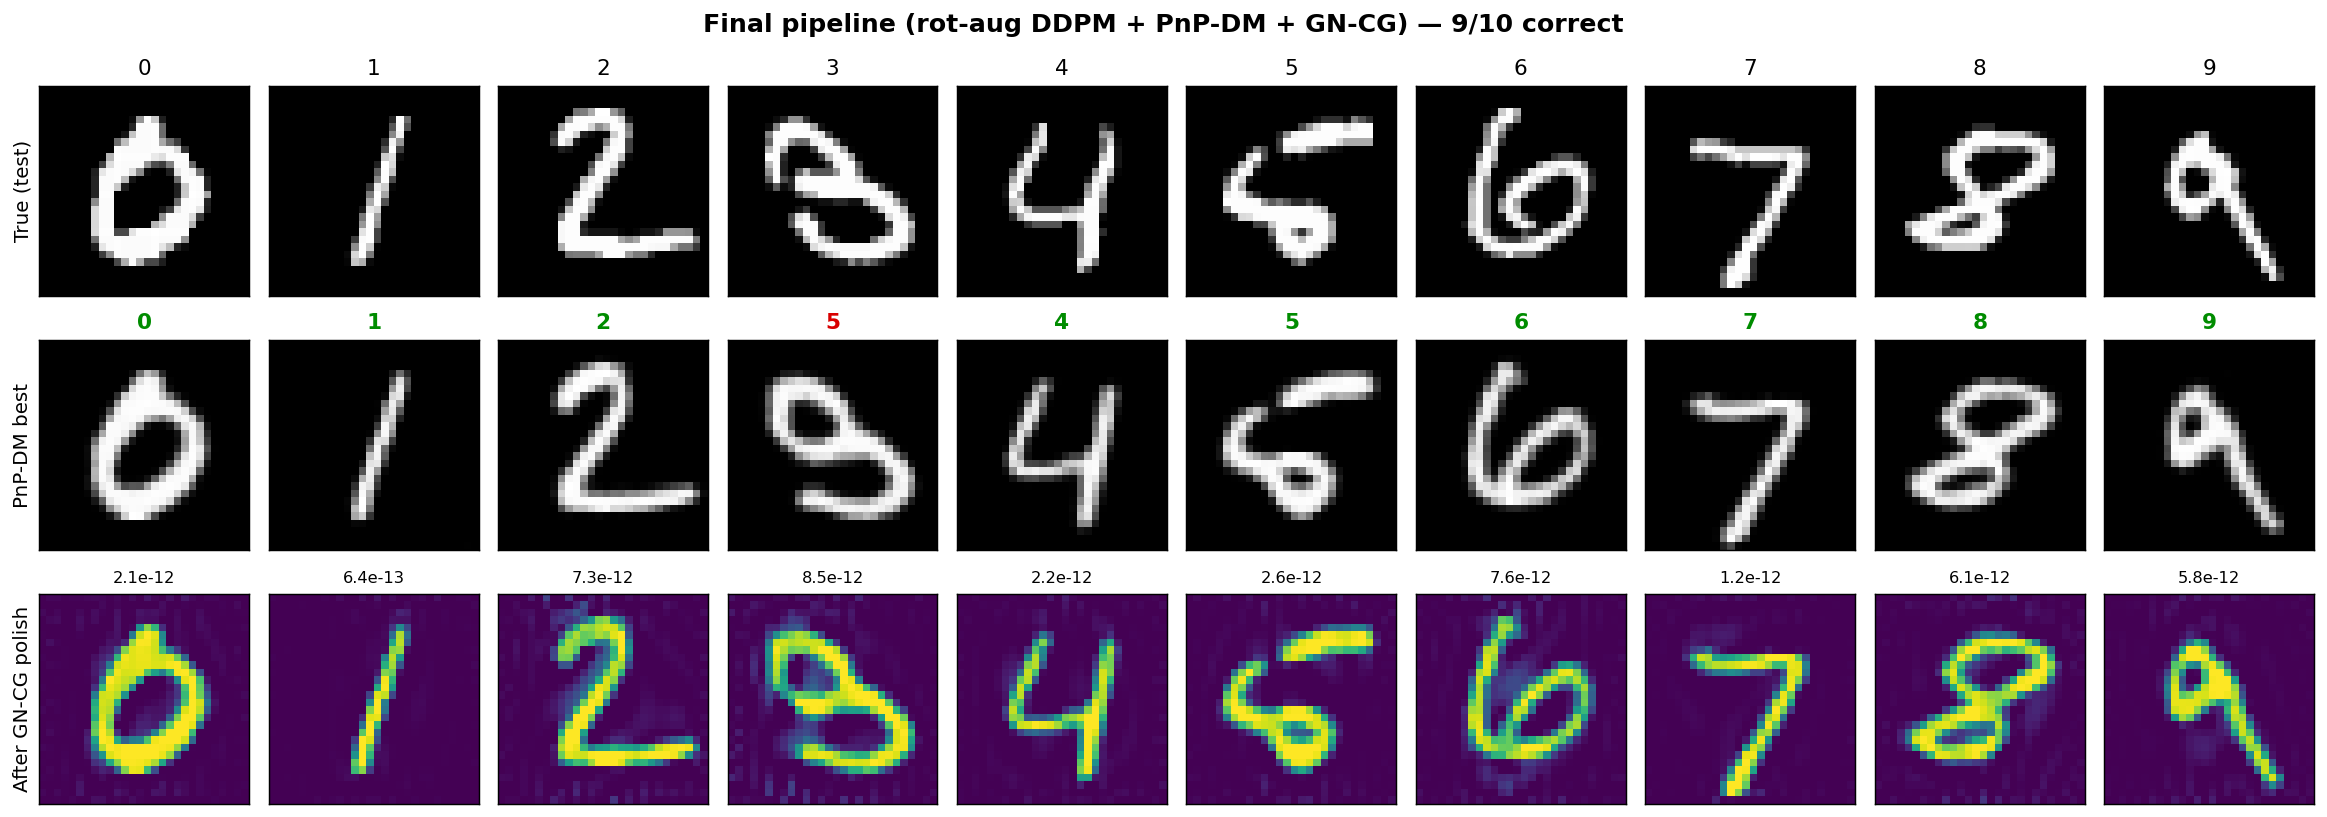
\includegraphics[width=0.95\linewidth]{validate_final.png}

\vspace{0.4em}
{\footnotesize
Labels read \textbf{true to recovered}. For each test digit we
synthesized fresh measurements, ran the full pipeline, and asked a
classifier to read the recovered image. The one miss (3 read as 5) is a
genuine ambiguity of the physics: that particular handwritten 3 has a
curled bottom that produces voltage readings extremely close to those of
certain 5s. The other nine cases polish to the same $10^{-12}$ regime
as the competition vector.}
\end{frame}

%==============================================================
\begin{frame}{Summary}
\footnotesize
\begin{itemize}\itemsep=4pt
\item Project 2 forced us off template matching and onto a diffusion
  prior. The first thing we tried, DPS, gave the wrong digit every time
  because its data step is too weak.
\item Variable splitting separates the two jobs. PnP-DM replaces the
  gradient nudge with a Gauss-Newton solve, which commits the chain to
  the right digit in a few iterations. 32 chains in parallel cover the
  posterior modes.
\item Rotation augmentation is a one-time twenty-minute fix that
  unlocks the diffusion prior for tilted digits.
\item A Newton-style polish replaces gradient descent at the endgame
  and drops the misfit by about five extra orders of magnitude.
\item \textbf{Result:} digit \textbf{5}, final misfit
  \textcolor{osuorange}{$6.16 \times 10^{-13}$}, held-out
  \textbf{9 out of 10}.
\end{itemize}

\vspace{0.6em}
\begin{center}
{\large\textcolor{osuorange}{\textbf{Thank you. Questions?}}}
\end{center}
\end{frame}

\end{document}
